\documentclass[11pt,a4paper]{article}

\usepackage[a4paper,margin=2.2cm]{geometry}
\usepackage[T1]{fontenc}
\usepackage[utf8]{inputenc}
\usepackage{lmodern}
\usepackage{microtype}
\usepackage{enumitem}
\usepackage{array}
\usepackage{amsmath}
\usepackage{amssymb}
\usepackage{booktabs}
\usepackage{tabularx}
\usepackage{titlesec}
\usepackage[table]{xcolor}
\usepackage{graphicx}
\usepackage{fancyhdr}
\usepackage{hyperref}
\usepackage{tikz}
\usetikzlibrary{shapes.geometric,positioning,decorations.pathmorphing,calc}
\usepackage{tcolorbox}
\tcbuselibrary{breakable,skins}

% ---------- Colors (course identity, matches tex/syllabus_010153103_1_2026.tex) ----------
\definecolor{kmutnbBlue}{HTML}{1F3A8A}
\definecolor{accent}{HTML}{0F6FC5}
\definecolor{lightGray}{HTML}{F2F4F7}
\definecolor{warn}{HTML}{B45309}
\definecolor{warnlight}{HTML}{FDF0E1}

% ---------- Line colors (for the schematic map and legend) ----------
\definecolor{lineSukhumvit}{HTML}{7AC943}
\definecolor{lineSilom}{HTML}{00693E}
\definecolor{lineBlue}{HTML}{114B9F}
\definecolor{linePurple}{HTML}{7A3B93}
\definecolor{lineInterchange}{HTML}{8A8A8A}

\hypersetup{
    colorlinks=true,
    linkcolor=accent,
    urlcolor=accent,
    citecolor=accent
}

\titleformat{\section}
  {\normalfont\large\bfseries\color{kmutnbBlue}}
  {\thesection}{0.6em}{}
\titleformat{\subsection}
  {\normalfont\bfseries\color{accent}}
  {\thesubsection}{0.6em}{}
\titlespacing*{\section}{0pt}{1.1\baselineskip}{0.35\baselineskip}
\titlespacing*{\subsection}{0pt}{0.8\baselineskip}{0.25\baselineskip}

\setlist[itemize]{leftmargin=1.4em,itemsep=2pt,topsep=2pt}
\setlist[enumerate]{leftmargin=1.6em,itemsep=2pt,topsep=2pt}

\pagestyle{fancy}
\fancyhf{}
\fancyhead[L]{\small\textit{010153103 Algorithms and Data Structures}}
\fancyhead[R]{\small Semester 1/2026}
\fancyfoot[C]{\small\thepage}
\renewcommand{\headrulewidth}{0.3pt}

% ---------- Note / gotcha callout box ----------
\newtcolorbox{gotcha}[1][Design Note]{
  enhanced,breakable,
  colback=warnlight,colframe=warn!80,
  title={\bfseries #1},
  fonttitle=\color{white},
  attach boxed title to top left={xshift=6pt,yshift=-3pt},
  boxed title style={colback=warn,boxrule=0pt,arc=2pt},
  arc=2pt,boxrule=0.4pt,
  top=12pt,
}

\begin{document}

%% ─── Title block ────────────────────────────────────────────────────────────
\begin{center}
  {\Large\bfseries\color{kmutnbBlue}
    Assignment 1/2026 --- Bangkok Transit Navigator: Web App Edition}\\[4pt]
  {\large\bfseries 010153103 \quad Algorithms and Data Structures}\\[2pt]
  {\normalsize Semester 1 / Academic Year 2026}\\[2pt]
  {\small Department of Electrical and Computer Engineering (ECE)}\\
  {\small Faculty of Engineering,
    King Mongkut's University of Technology North Bangkok}
\end{center}

\noindent\rule{\linewidth}{0.4pt}\medskip

\noindent
This assignment builds on the graph and shortest-path concepts from
Lectures~18--19 (Graphs, Shortest Paths). If you have not yet reviewed
those lectures, do that first --- this assignment assumes you already know
the Graph ADT, Dijkstra's algorithm, and priority queues.

%% ─── 1. Scenario ────────────────────────────────────────────────────────────
\section{Scenario}

You will build a small web application, the \textbf{Bangkok Transit
Navigator}, that lets a rider:

\begin{enumerate}
  \item Enter an \textbf{origin} and \textbf{destination} station.
  \item Enter either a \textbf{departure time} (``I'm leaving at 08:15,
        when do I arrive?'') or a \textbf{desired arrival time} (``I need
        to be there by 09:00, when should I leave?'').
  \item Choose how the route should be optimized: \textbf{fastest total
        time}, or \textbf{fewest interchanges}.
  \item See the resulting itinerary as both text (stop-by-stop) and a
        \textbf{line-colored map} with the chosen route highlighted.
\end{enumerate}

This is a full application with a graph engine and a browser-based UI, and
it must reason about \emph{time}, not just hop count.

%% ─── 2. Learning Objectives ─────────────────────────────────────────────────
\section{Learning Objectives}
\begin{itemize}
  \item Build a weighted graph from a real-world, imperfectly-structured CSV file.
  \item Model a genuinely tricky real-world constraint (line-transfer penalties)
        as a graph modeling problem, not just an algorithm problem.
  \item Implement Dijkstra's algorithm with \textbf{two different cost functions}
        (time vs.\ interchange count) against the same underlying graph.
  \item Render a graph visually, using line identity (color) as the primary
        visual encoding.
  \item Design a small, usable UI on top of a correct backend algorithm.
\end{itemize}

%% ─── 3. Provided Data ───────────────────────────────────────────────────────
\section{Provided Data}

File: \texttt{assignment/bangkok\_transit/bangkok\_network\_graph.csv}

\renewcommand{\arraystretch}{1.25}
\begin{tabularx}{\linewidth}{@{}l X@{}}
  \toprule
  \rowcolor{kmutnbBlue!90}
  \textcolor{white}{\textbf{Column}} & \textcolor{white}{\textbf{Meaning}} \\
  \midrule
  \texttt{Source\_Station\_Code} & Unique code for the source \emph{platform} (e.g. \texttt{N8}, \texttt{BL12}) \\
  \rowcolor{lightGray}
  \texttt{Source\_Station\_Name} & Human-readable name (e.g. Mo Chit) \\
  \texttt{Target\_Station\_Code} & Unique code for the target platform \\
  \rowcolor{lightGray}
  \texttt{Target\_Station\_Name} & Human-readable name \\
  \texttt{Edge\_Type} & \texttt{Line Track} (ride between adjacent stations on one line) or \texttt{Interchange Connection} (walk between platforms to change lines) \\
  \rowcolor{lightGray}
  \texttt{Line\_Context} & Which line the edge belongs to, e.g.\ \texttt{BTS Sukhumvit Line}, \texttt{MRT Blue Line}, or a description of which two lines an interchange connects \\
  \bottomrule
\end{tabularx}

\medskip
\noindent\textbf{Read the whole file before you start coding.} It has a few
properties that will matter for your design:

\begin{itemize}
  \item \textbf{Station codes are the real identity, not names.} Several
        physical interchange stations are represented by \emph{two different
        codes} for the same location --- e.g.\ Bang Wa is \texttt{S12} (BTS
        Silom) and \texttt{BL33} (MRT Blue); Sukhumvit is \texttt{E4} (BTS)
        and \texttt{BL21} (MRT); Tao Poon is \texttt{BL09} (MRT Blue) and
        \texttt{PP16} (MRT Purple). Build your graph keyed on \emph{code},
        and only use the name for display.
  \item \textbf{\texttt{Line Track} rows are listed once per direction} as
        the line was traced, but riders can travel either way along the
        track. Decide how you will represent that (e.g.\ treat the graph as
        undirected, or insert both directions when you parse each row) and
        be consistent.
  \item \textbf{The MRT Blue Line is not a simple line} --- it has a loop
        and a branch. Trace it on paper before you code: \texttt{BL01} (Tha
        Phra) closes a loop back to itself via \texttt{BL31}, and also
        branches off towards \texttt{BL37} (Lak Song). Your graph
        representation must support this without special-casing it.
  \item \textbf{The dataset has a minor duplicate.} The edge between
        \texttt{BL01} and \texttt{BL32} appears twice, once tagged
        \texttt{MRT Blue Line} and once \texttt{MRT Blue Line Branch}. This
        is a realistic data-quality quirk, not a bug in the assignment ---
        decide whether to de-duplicate it and say so in your report.
  \item \textbf{One row is a self-loop:}
        \texttt{CEN,Siam,CEN,Siam,Interchange Connection,Cross-Platform
        Interchange (Sukhumvit <-> Silom)}. Read section~\ref{sec:gotcha}
        before deciding how to handle it --- it is the single most
        important modeling decision in this assignment.
\end{itemize}

%% ─── 4. Part 1 ──────────────────────────────────────────────────────────────
\section{Part 1 --- Build the Graph}
\begin{itemize}
  \item Parse the CSV into an in-memory graph using the Graph ADT style from
        Lecture~18 (vertices and edges as objects, adjacency list keyed by
        vertex).
  \item Vertices are station \emph{codes}; store the display name and line
        as vertex attributes.
  \item In your report, justify your choice of adjacency list vs.\
        adjacency matrix in terms of the network's sparsity (count the
        vertices and edges and say so explicitly).
\end{itemize}

%% ─── 5. Part 2: Visualize ───────────────────────────────────────────────────
\section{Part 2 --- Visualize the Network}

Render every station and every \texttt{Line Track} edge, with \textbf{each
line drawn in a distinct, consistent color}:

\renewcommand{\arraystretch}{1.3}
\begin{tabularx}{\linewidth}{@{}l X@{}}
  \toprule
  \rowcolor{kmutnbBlue!90}
  \textcolor{white}{\textbf{Line}} & \textcolor{white}{\textbf{Suggested color}} \\
  \midrule
  BTS Sukhumvit Line & \tikz\draw[lineSukhumvit,line width=4pt] (0,0) -- (0.9,0); \ Light green \\
  \rowcolor{lightGray}
  BTS Silom Line & \tikz\draw[lineSilom,line width=4pt] (0,0) -- (0.9,0); \ Dark green \\
  MRT Blue Line (incl.\ branch) & \tikz\draw[lineBlue,line width=4pt] (0,0) -- (0.9,0); \ Blue \\
  \rowcolor{lightGray}
  MRT Purple Line & \tikz\draw[linePurple,line width=4pt] (0,0) -- (0.9,0); \ Purple (only the \texttt{PP16} connection point appears in the data) \\
  Interchange Connection edges & \tikz\draw[lineInterchange,line width=2pt,dashed] (0,0) -- (0.9,0); \ Neutral grey, dashed --- reads as ``walk here,'' not ``ride here'' \\
  \bottomrule
\end{tabularx}

\medskip
\noindent You do \textbf{not} need real geographic coordinates. A clean,
readable layout (e.g.\ laying each line out as a path/loop and placing
interchange edges as short connectors between them) is perfectly
acceptable --- the grading criterion is that a viewer can tell, at a
glance, which line is which and where the transfer points are. Client-side
visualization libraries (D3.js, Cytoscape.js, vis-network, or even
hand-rolled SVG/Canvas) are all fine here --- see the constraints in
section~\ref{sec:constraints}. The graph-building and pathfinding code must
be your own.

\begin{figure}[htbp]
\centering
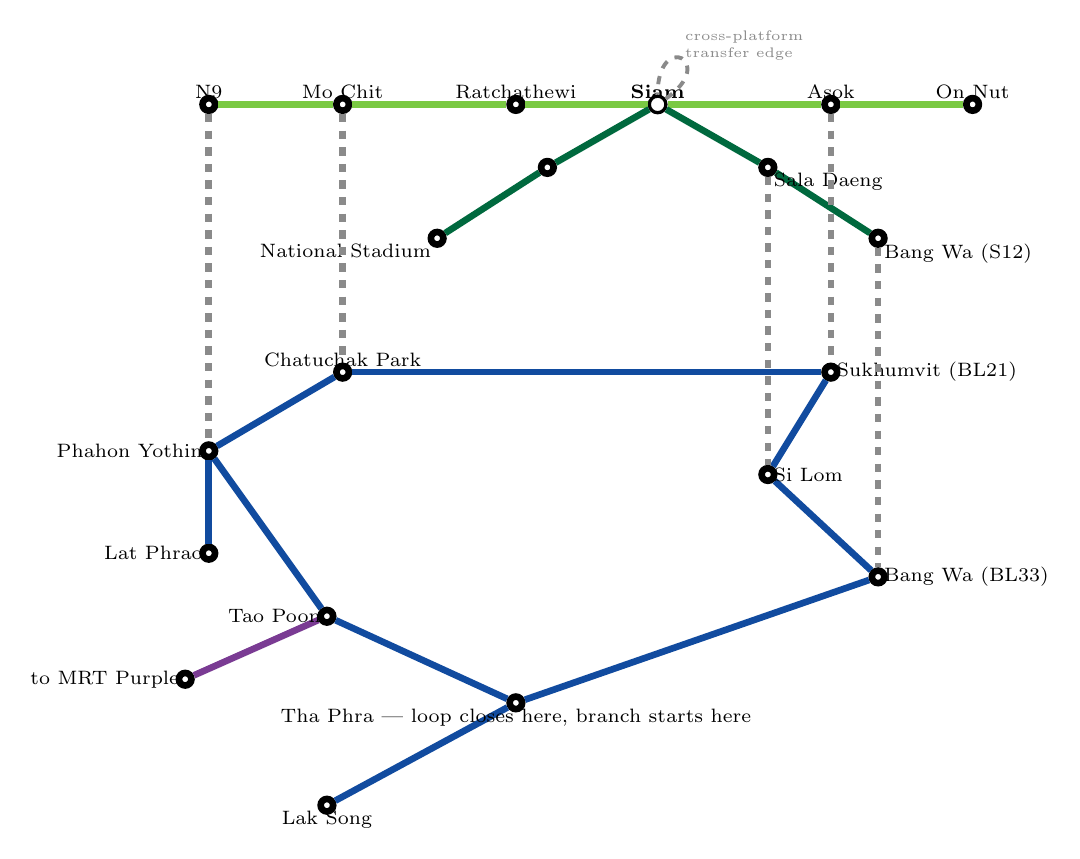
\begin{tikzpicture}[
  station/.style={circle,draw=black,fill=white,inner sep=1.6pt,minimum size=4pt},
  interchange/.style={circle,draw=black,fill=white,line width=1.2pt,inner sep=2pt,minimum size=6pt},
  lbl/.style={font=\scriptsize,inner sep=1pt},
  every path/.style={line width=2.4pt}
]
  % --- BTS Sukhumvit Line (top row, light green) ---
  \node[station]     (N9)  at (0.5,7)  {};
  \node[station]     (N8)  at (2.2,7)  {};
  \node[station]     (N1)  at (4.4,7)  {};
  \node[interchange] (CEN) at (6.2,7)  {};
  \node[station]     (E4)  at (8.4,7)  {};
  \node[station]     (E9)  at (10.2,7) {};
  \draw[lineSukhumvit] (N9) -- (N8) -- (N1) -- (CEN) -- (E4) -- (E9);
  \node[lbl,above] at (N9)  {N9};
  \node[lbl,above] at (N8)  {Mo Chit};
  \node[lbl,above] at (N1)  {Ratchathewi};
  \node[lbl,above,font=\scriptsize\bfseries] at (CEN) {Siam};
  \node[lbl,above] at (E4)  {Asok};
  \node[lbl,above] at (E9)  {On Nut};

  % --- Cross-platform self-loop at Siam: drawn as a visible small loop, offset to a clear area ---
  \draw[lineInterchange,dashed,line width=1.4pt] (CEN) to[out=35,in=90,looseness=18] (CEN);
  \node[lbl,lineInterchange,align=left,font=\tiny] at (7.3,7.75) {cross-platform\\transfer edge};

  % --- BTS Silom Line (diagonal from Siam, dark green) ---
  \node[station] (W1)  at (3.4,5.3) {};
  \node[station] (S1x) at (4.8,6.2) {};
  \node[station] (S2x) at (7.6,6.2) {};
  \node[station] (S12) at (9.0,5.3) {};
  \draw[lineSilom] (W1) -- (S1x) -- (CEN) -- (S2x) -- (S12);
  \node[lbl,below left]  at (W1)  {National Stadium};
  \node[lbl,below right] at (S2x) {Sala Daeng};
  \node[lbl,below right] at (S12) {Bang Wa (S12)};

  % --- MRT Blue Line: loop + branch (blue), positioned below ---
  \node[station] (BL12) at (2.2,3.6)  {}; % Chatuchak Park -- under N8
  \node[station] (BL13) at (0.5,2.6)  {}; % Phahon Yothin -- under N9
  \node[station] (BL14) at (0.5,1.3)  {}; % Lat Phrao
  \node[station] (BL21) at (8.4,3.6)  {}; % Sukhumvit -- under E4
  \node[station] (BL25) at (7.6,2.3)  {}; % Si Lom -- under S2x
  \node[station] (BL33) at (9.0,1.0)  {}; % Bang Wa -- under S12
  \node[station] (BL01) at (4.4,-0.6) {}; % Tha Phra (loop closure + branch point)
  \node[station] (BL09) at (2.0,0.5)  {}; % Tao Poon
  \node[station] (BL37) at (2.0,-1.9) {}; % Lak Song (branch end)
  \node[station] (PP16) at (0.2,-0.3) {}; % Purple Line connection

  \draw[lineBlue] (BL12) -- (BL21);
  \draw[lineBlue] (BL21) -- (BL25) -- (BL33);
  \draw[lineBlue] (BL33) -- (BL01);
  \draw[lineBlue] (BL01) -- (BL09) -- (BL13) -- (BL12);
  \draw[lineBlue] (BL13) -- (BL14);
  \draw[lineBlue] (BL01) -- (BL37);
  \draw[linePurple] (BL09) -- (PP16);

  \node[lbl,left]  at (BL13) {Phahon Yothin};
  \node[lbl,left]  at (BL14) {Lat Phrao};
  \node[lbl,above] at (BL12) {Chatuchak Park};
  \node[lbl,right] at (BL21) {Sukhumvit (BL21)};
  \node[lbl,right] at (BL25) {Si Lom};
  \node[lbl,right] at (BL33) {Bang Wa (BL33)};
  \node[lbl,below] at (BL01) {Tha Phra --- loop closes here, branch starts here};
  \node[lbl,left]  at (BL09) {Tao Poon};
  \node[lbl,below] at (BL37) {Lak Song};
  \node[lbl,left]  at (PP16) {to MRT Purple};

  % --- Interchange connectors (grey dashed) between distinct codes ---
  \draw[lineInterchange,dashed] (N8) -- (BL12);
  \draw[lineInterchange,dashed] (N9) -- (BL13);
  \draw[lineInterchange,dashed] (E4) -- (BL21);
  \draw[lineInterchange,dashed] (S2x) -- (BL25);
  \draw[lineInterchange,dashed] (S12) -- (BL33);
\end{tikzpicture}
\caption{Simplified schematic of the network (not all 60+ stations shown;
line colors match the table above), illustrating the Blue Line loop and
its branch to Lak Song, ordinary interchange links (dashed grey) between
distinct station codes, and the Siam cross-platform self-loop (dashed
loop at \texttt{CEN}). Your submission's map should cover the full CSV.}
\label{fig:map}
\end{figure}

\subsection{Highlighting a computed route}
Once Part~4 is working, the same visualization must be able to highlight a
computed itinerary on top of the full map (e.g.\ thicker/bolder stroke on
the traveled edges, and markers on the boarding/alighting/interchange
stations).

%% ─── 6. Part 3: Weighting ───────────────────────────────────────────────────
\section{Part 3 --- Weighting the Graph}

You must assign a \textbf{time cost} to every edge:
\begin{itemize}
  \item \textbf{\texttt{Line Track} edges:} the CSV has no travel-time
        column, so you must choose and justify a constant per-segment
        time. A reasonable default is \textbf{2.5--3 minutes} between
        adjacent stations (typical BTS/MRT scheduled time) --- you may use
        a different number if you justify it.
  \item \textbf{\texttt{Interchange Connection} edges between two different
        station codes} (e.g.\ \texttt{E4}~$\leftrightarrow$~\texttt{BL21},
        \texttt{S2}~$\leftrightarrow$~\texttt{BL25},
        \texttt{N8}~$\leftrightarrow$~\texttt{BL12},
        \texttt{N9}~$\leftrightarrow$~\texttt{BL13},
        \texttt{S12}~$\leftrightarrow$~\texttt{BL33},
        \texttt{BL09}~$\leftrightarrow$~\texttt{PP16}): these represent a
        real walk between separate platforms/buildings. A reasonable
        default penalty is \textbf{5--7 minutes}.
\end{itemize}

\subsection{The Siam gotcha --- read this before you code}
\label{sec:gotcha}

\begin{gotcha}[The Siam ({\ttfamily CEN}) Gotcha]
At Siam, both the Sukhumvit and Silom lines use the \textbf{same vertex
code}, \texttt{CEN}. That means a naive graph walk from, say, \texttt{N1}
(Ratchathewi) to \texttt{S1} (Ratchadamri) can pass straight through
\texttt{CEN} --- arriving on one line and leaving on the other --- \textbf{without
ever being forced to use the \texttt{CEN}$\to$\texttt{CEN} self-loop edge},
because \texttt{CEN} already connects directly to both \texttt{N1} and
\texttt{S1}. If your shortest-path algorithm only tracks ``which station am
I at,'' it will silently give this transfer a cost of zero, which is wrong:
a rider here really does have to cross to the opposite platform.

You need a strategy that reliably charges the cross-platform penalty
whenever a path's \texttt{Line\_Context} changes at \texttt{CEN}, and ---
for consistency --- you should think about whether the same strategy also
correctly counts an interchange for the fewest-interchanges optimization
mode (section~\ref{sec:optmode}). Two directions worth considering:
\begin{itemize}
  \item Track \textbf{which line the rider is currently on} as part of your
        search state (e.g.\ search over \texttt{(station\_code,
        current\_line)} pairs instead of bare station codes), so that
        arriving at \texttt{CEN} on the Sukhumvit line and leaving on the
        Silom line is a detectable, chargeable transition --- the same
        technique naturally also covers the explicit \texttt{Interchange
        Connection} edges elsewhere in the network.
  \item Or, keep the simpler bare-station-code graph and add explicit
        bookkeeping in your path-reconstruction step that specifically
        detects a \texttt{Line\_Context} change at \texttt{CEN}.
\end{itemize}
Either is acceptable. What is \textbf{not} acceptable is a route through
Siam that silently costs nothing to change lines. Explain and justify
whichever approach you took in your report.
\end{gotcha}

%% ─── 7. Part 4: Web App ─────────────────────────────────────────────────────
\section{Part 4 --- The Web App}

\subsection{Departure mode}
Given an origin, destination, and a departure time (\texttt{HH:MM}),
compute the shortest-cost path and report:
\begin{itemize}
  \item Estimated \textbf{arrival time} = departure time + total travel
        time along the path.
  \item The full itinerary (see~\ref{sec:ui}).
\end{itemize}

\subsection{Arrival mode}
Given an origin, destination, and a \textbf{desired arrival time}, compute
the same shortest path and report the \textbf{latest departure time} that
still meets it: $\text{departure} = \text{arrival} - \text{total travel
time}$.

\begin{gotcha}[Note]
Because this dataset has no train schedule/frequency information, edge
weights don't depend on time of day, so ``plan by arrival'' is
intentionally the mirror image of ``plan by departure'' rather than a
separate search. If you want a harder version of this, see the bonus in
section~\ref{sec:bonus}.
\end{gotcha}

\subsection{Optimization mode}
\label{sec:optmode}
The user must be able to choose between two objectives, computed against
the \textbf{same graph}:
\begin{itemize}
  \item \textbf{Fastest route:} minimize total time (as weighted in
        section~6).
  \item \textbf{Fewest interchanges:} minimize the number of line changes;
        use total time only to break ties between routes with the same
        number of interchanges.
\end{itemize}
Implement this as two different cost functions/comparators feeding the
same Dijkstra implementation (or two clearly related variants) --- don't
just hard code two unrelated algorithms. Your report should explain how
you adapted Dijkstra (or, if you chose it, a different single-source
shortest-path approach) for the fewest-interchanges objective, and how
you're counting an interchange consistently with your answer to
section~\ref{sec:gotcha}.

\subsection{UI requirements}
\label{sec:ui}
\begin{itemize}
  \item Origin/destination pickers (autocomplete or dropdown over station
        names --- remember several names map to more than one code; if the
        user picks an interchange station by name, either ask which
        platform or treat it as ``already there,'' whichever you justify).
  \item A time input, and a toggle between ``Depart at'' / ``Arrive by.''
  \item A toggle between ``Fastest'' / ``Fewest interchanges.''
  \item Output: a stop-by-stop itinerary --- e.g.\ \emph{``Board BTS
        Sukhumvit Line at Mo Chit (08:15) $\rightarrow$ ride to Siam
        (08:32) $\rightarrow$ cross platform to BTS Silom Line (08:35)
        $\rightarrow$ ride to Sala Daeng (08:44). Total: 29 min, 1
        interchange.''} --- plus the highlighted map from
        Figure~\ref{fig:map}.
  \item Basic error handling: identical origin/destination, unknown
        station, malformed time.
\end{itemize}

\begin{figure}[h]
\centering
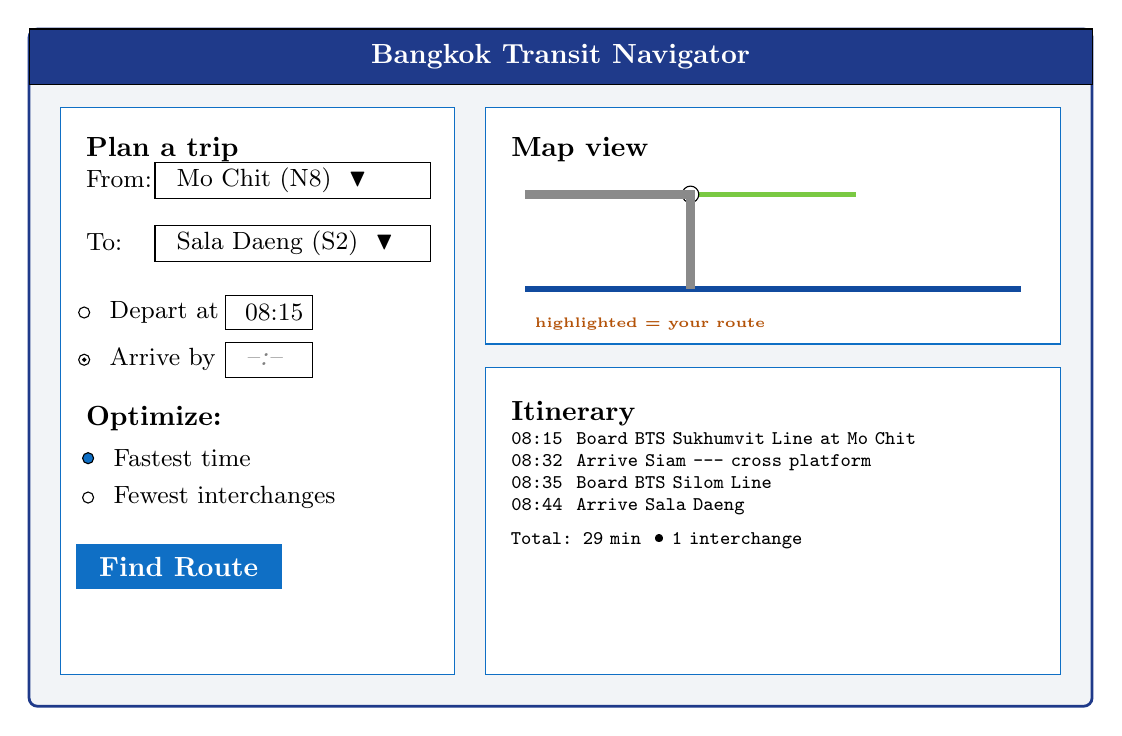
\begin{tikzpicture}[font=\small]
  % Outer app frame
  \draw[draw=kmutnbBlue,fill=lightGray,line width=1pt,rounded corners=3pt] (0,0) rectangle (13.5,8.6);
  % Title bar
  \draw[fill=kmutnbBlue] (0,7.9) rectangle (13.5,8.6);
  \node[white,font=\bfseries] at (6.75,8.25) {Bangkok Transit Navigator};

  % Left control panel
  \draw[fill=white,draw=accent] (0.4,0.4) rectangle (5.4,7.6);
  \node[anchor=north west,font=\bfseries] at (0.6,7.35) {Plan a trip};

  \node[anchor=west] at (0.6,6.7) {From:};
  \draw[draw=black] (1.6,6.45) rectangle (5.1,6.9);
  \node[anchor=west] at (1.75,6.675) {Mo Chit (N8) \ \small$\blacktriangledown$};

  \node[anchor=west] at (0.6,5.9) {To:};
  \draw[draw=black] (1.6,5.65) rectangle (5.1,6.1);
  \node[anchor=west] at (1.75,5.875) {Sala Daeng (S2) \ \small$\blacktriangledown$};

  \draw[draw=black,fill=white] (0.7,5.0) circle (0.07);
  \node[anchor=west] at (0.9,5.0) {Depart at};
  \draw[draw=black] (2.5,4.78) rectangle (3.6,5.22);
  \node[anchor=west] at (2.62,5.0) {08:15};

  \draw[draw=black,fill=black] (0.7,4.4) circle (0.02);
  \draw[draw=black] (0.7,4.4) circle (0.07);
  \node[anchor=west] at (0.9,4.4) {Arrive by};
  \draw[draw=black] (2.5,4.18) rectangle (3.6,4.62);
  \node[anchor=west,font=\itshape,color=black!50] at (2.62,4.4) {--:--};

  \node[anchor=west,font=\bfseries] at (0.6,3.65) {Optimize:};
  \draw[draw=black,fill=accent] (0.75,3.15) circle (0.07);
  \node[anchor=west] at (0.95,3.15) {Fastest time};
  \draw[draw=black] (0.75,2.65) circle (0.07);
  \node[anchor=west] at (0.95,2.65) {Fewest interchanges};

  \draw[fill=accent,draw=accent] (0.6,1.5) rectangle (3.2,2.05);
  \node[white,font=\bfseries] at (1.9,1.775) {Find Route};

  % Right panel: map view
  \draw[fill=white,draw=accent] (5.8,4.6) rectangle (13.1,7.6);
  \node[anchor=north west,font=\bfseries] at (6.0,7.35) {Map view};
  \draw[lineSukhumvit,line width=2pt] (6.3,6.5) -- (10.5,6.5);
  \draw[lineSilom,line width=2pt] (8.4,6.5) -- (8.4,5.3);
  \draw[lineBlue,line width=2pt] (6.3,5.3) -- (12.6,5.3);
  \node[circle,draw=black,fill=white,minimum size=6pt,inner sep=1pt] at (8.4,6.5) {};
  \draw[lineInterchange,line width=3pt] (6.3,6.5) -- (8.4,6.5) -- (8.4,5.3);
  \node[font=\tiny,anchor=west,color=warn] at (6.3,4.85) {\bf highlighted = your route};

  % Right panel: itinerary output
  \draw[fill=white,draw=accent] (5.8,0.4) rectangle (13.1,4.3);
  \node[anchor=north west,font=\bfseries] at (6.0,4.0) {Itinerary};
  \node[anchor=north west,align=left,font=\ttfamily\scriptsize,text width=6.9cm] at (6.0,3.6) {
    08:15 \ Board BTS Sukhumvit Line at Mo Chit\\
    08:32 \ Arrive Siam --- cross platform\\
    08:35 \ Board BTS Silom Line\\
    08:44 \ Arrive Sala Daeng\\[4pt]
    \textbf{Total: 29 min \ \textbullet\ 1 interchange}
  };
\end{tikzpicture}
\caption{Illustrative wireframe of the required UI elements: station
pickers, departure/arrival toggle, optimization toggle, a highlighted map
view, and a stop-by-stop itinerary with total time and interchange count.
Visual styling is entirely up to you --- only the elements shown are
required.}
\label{fig:ui}
\end{figure}

%% ─── 8. Constraints ─────────────────────────────────────────────────────────
\section{Technical Constraints}
\label{sec:constraints}
\begin{itemize}
  \item \textbf{You must implement the graph, Dijkstra's algorithm (or
        your chosen shortest-path algorithm), and the priority queue
        yourself.} Do not call a library's built-in shortest-path or
        graph-routing function --- that is the part of this assignment
        being assessed.
  \item Any language/stack is fine (e.g.\ vanilla JavaScript/TypeScript in
        the browser; a small Node/Express, Java, or Python backend with an
        HTML/JS frontend). Pick whichever lets you finish; a simple
        single-page client-side app is entirely sufficient.
  \item For \textbf{rendering only} (drawing the map, laying out nodes, UI
        widgets), third-party libraries are fine --- that part isn't the
        DSA content of this assignment.
\end{itemize}

%% ─── 9. Deliverables ────────────────────────────────────────────────────────
\section{Deliverables}
\begin{itemize}
  \item \textbf{Source code}, organized and readable, with instructions to
        run it locally (e.g.\ \texttt{README.md} with setup steps).
  \item \textbf{Report} covering: your name and student ID; graph
        representation choice and sparsity justification; how you modeled
        and charged interchange penalties, including your answer to the
        Siam (\texttt{CEN}) gotcha; how you adapted Dijkstra for the
        fewest-interchanges objective; the travel-time and
        interchange-penalty constants you chose and why; and any
        data-cleaning decisions (e.g.\ the \texttt{BL01}$\leftrightarrow$\texttt{BL32}
        duplicate).
  \item \textbf{Example runs} (screenshots or text) for the test cases in
        section~\ref{sec:tests}.
\end{itemize}

%% ─── 10. Rubric ─────────────────────────────────────────────────────────────
\section{Grading Rubric}
\renewcommand{\arraystretch}{1.3}
\rowcolors{2}{lightGray}{white}
\begin{tabularx}{\linewidth}{X >{\centering\arraybackslash}p{2.2cm}}
  \toprule
  \rowcolor{kmutnbBlue!90}
  \textcolor{white}{\textbf{Criterion}} & \textcolor{white}{\textbf{Weight}} \\
  \midrule
  Graph correctly built from the CSV (handles codes vs.\ names, the loop/branch, direction) & 20\% \\
  Correct time-weighted shortest path, both departure and arrival modes & 20\% \\
  Correct fewest-interchanges mode, including the Siam case & 20\% \\
  Visualization: lines colored and distinguishable, route highlighting works & 15\% \\
  Report: clear justification of design decisions above & 15\% \\
  UI usability \& error handling & 10\% \\
  \bottomrule
\end{tabularx}
\rowcolors{1}{}{}

%% ─── 11. Example Test Cases ─────────────────────────────────────────────────
\section{Example Test Cases}
\label{sec:tests}
Verify your app against at least these routes (exact times will depend on
your chosen constants --- what's graded is that the logic and interchange
count are correct):

\begin{enumerate}
  \item \textbf{Bang Wa (\texttt{S12}/\texttt{BL33}) $\to$ Lat Phrao
        (\texttt{BL14})} --- exercises the BTS$\leftrightarrow$MRT
        interchange at Bang Wa and the MRT Blue Line loop/branch.
  \item \textbf{Lak Song (\texttt{BL37}) $\to$ Kheha (\texttt{E23})} --- a
        long cross-network trip, traversing most of the Blue Line then
        most of the Sukhumvit Line.
  \item \textbf{Ratchathewi (\texttt{N1}) $\to$ National Stadium
        (\texttt{W1})} --- the Siam gotcha: this route must reflect a
        cross-platform interchange cost at \texttt{CEN}, not a free
        pass-through.
  \item Any pair of your choosing, once in \textbf{``fastest''} mode and
        once in \textbf{``fewest interchanges''} mode, where the two modes
        give a \emph{different} route --- to demonstrate the modes are
        genuinely independent.
\end{enumerate}

%% ─── 12. Bonus ──────────────────────────────────────────────────────────────
\section{Bonus Challenges (optional, extra credit)}
\label{sec:bonus}
\begin{itemize}
  \item \textbf{Train frequency / headway:} instead of instant transfers,
        assume each line runs every $N$ minutes and add an expected wait
        time when boarding or transferring --- this makes ``plan by
        arrival'' genuinely asymmetric with ``plan by departure,'' unlike
        the base assignment.
  \item \textbf{First/last train:} model service hours and reject or
        adjust queries outside them.
  \item \textbf{Station closure:} let the user mark a station ``closed for
        maintenance'' and recompute the best detour.
  \item \textbf{Shareable route:} encode a computed trip in the URL so it
        can be copied and reopened directly to that result.
\end{itemize}

%% ─── 13. AI Collaboration ───────────────────────────────────────────────────
\section{AI Collaboration}
You may use an AI assistant to discuss graph-modeling approaches (e.g.\
``how do I represent a rider's current line as part of a Dijkstra search
state?'') or to debug. You may not have it design your whole solution for
you, and you must be able to explain, live, any part of your submitted
code --- this includes your justification for how you handled the Siam
interchange case. Disclose any significant AI assistance in your report.

%% ─── 14. Submission ─────────────────────────────────────────────────────────
\section{Submission}
Submit your source code repository link (or archive) and report PDF via
the course site by the announced deadline.

\bigskip
\noindent\rule{\linewidth}{0.4pt}
\begin{center}
  \small\textit{This assignment is subject to minor adjustments at the
  instructor's discretion. Students are responsible for staying informed
  of any changes announced in class or via the course website.}
\end{center}

\end{document}
